\section{Procedimiento}

\subsection{Pruebas de vacío}
Se realizó por el lado de baja tensión (BT) dejando el lado de alta tensión (AT) en vacío es decir, sin carga conectada

\begin{figure}[h!] % [h!] significa "aquí", puedes cambiarlo por t=top, b=bottom
    \centering
    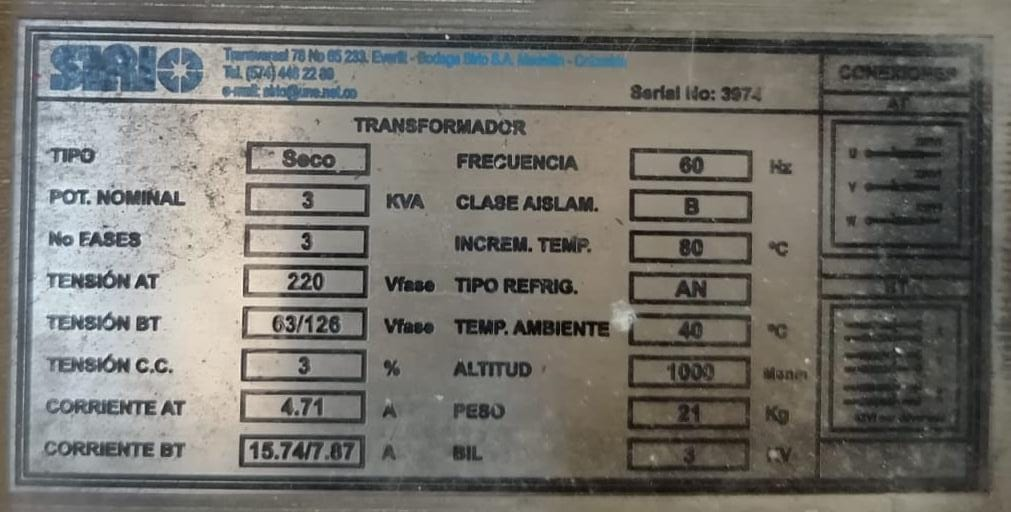
\includegraphics[width=0.48\textwidth]{figs/placa_datos.jpeg} % ajusta el ancho
    \caption{Placa de datos transformador}
    \label{fig:mi_imagen}
\end{figure}

La tensión nóminal por fase en el devanado de BT es 126 V, por lo tanto: 

\[
V_{\text{línea}} = \sqrt{3}\,V_{\text{fase}} = \sqrt{3}\cdot 126 \approx 218.18\ \mathrm{V}
\]

Esta tensión fue el valor aplicado en la fuente.


Datos medidos:

\begin{itemize}
    \item Potencia
\[
P_0 = 3 \ \text{W}
\]
\item Corriente
\[
I_0 = 0.18 \ \text{A}
\]
\end{itemize}

Con esto es posible hallar los parámetros de la rama de magnetización

\[
\theta = \cos^{-1}\!\left(\frac{P}{\sqrt{3} \, V_{ac} \, I_{ac}}\right) = 87.4722^\circ
\]

\[
Y_m = \frac{I_{ac}}{V_{ac}} \angle \theta = \frac{0.18}{218.8} \angle 87.4722^\circ
\]

\[
Y_m = 3.638 \times 10^{-5} + j\,8.242 \times 10^{-4} \; = G + jB
\]


\[
R_m = \frac{1}{G} = 2.7483 \times 10^{4}
\qquad
X_m = \frac{1}{B} = 1.2133 \times 10^{3}
\]






\section{Prueba de Cortocircuito}
La \textbf{prueba de cortocircuito} permite determinar los parámetros de la impedancia equivalente del transformador. A continuación, se presentan las mediciones realizadas cuando el transformador fue alimentado por el lado de alta tensión (AT).

\begin{table}[h!]
\centering
\caption{Medidas de la prueba de cortocircuito.}
\begin{tabular}{|c|c|c|}
\hline
Tensión (V) & Corriente (A) & Potencia (W) \\ \hline
4.71 & 19.5 & 150 \\ \hline
\end{tabular}
\end{table}

A partir de las pruebas de cortocircuito es posible calcular los parámetros de la impedancia equivalente del transformador, tal como se muestra a continuación.

\vspace{1em}
Con los resultados de las pruebas de vacío y cortocircuito ya obtenidos, se determinaron todos los parámetros esenciales para construir el \textbf{circuito equivalente}, el cual se representa en la siguiente figura:

\begin{figure}[h!] % [h!] significa "aquí", puedes cambiarlo por t=top, b=bottom
    \centering
    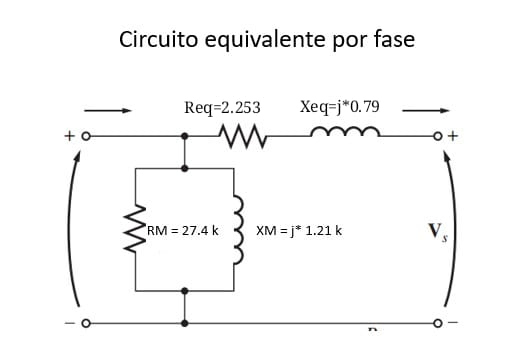
\includegraphics[width=0.48\textwidth]{figs/CE.jpeg} % ajusta el ancho
    \caption{\textit{(Imagen del modelo del circuito equivalente)}}
    \label{fig:mi_imagen1}
\end{figure}


\section{Prueba de regulación con diferentes cargas eléctricas}

La \textbf{regulación de voltaje} en un transformador trifásico mide la variación del voltaje secundario cuando el transformador pasa de estar sin carga (en vacío) a con carga nominal. En condiciones ideales, el transformador mantendría constante su tensión secundaria; sin embargo, debido a las caídas internas de tensión en la resistencia y reactancia de los devanados, el voltaje varía cuando se conecta una carga.

El cálculo de la regulación porcentual de voltaje se realiza mediante la expresión:

\begin{equation}
    \label{eq:regulacion} % Etiqueta para referenciar la ecuación correctamente
    \text{Regulación (\%)} = \frac{V_{sc} - V_c}{V_c} \times 100
\end{equation}

Para las pruebas se emplearon los bancos de cargas monofásicos del laboratorio, cuyas características se resumen en la Tabla~\ref{tab:cargas}.

\begin{table} % Se quita [H] para evitar problemas de flotación con el formato IEEE
\centering
\caption{Cargas del laboratorio de Máquinas Eléctricas monofásica}
\label{tab:cargas}
\footnotesize
\setlength{\tabcolsep}{2.5pt} % Reduce espacio entre columnas
\begin{tabular}{|l|c|c|c|}
\hline
\textbf{Carga} & \textbf{Posición} & \textbf{Elemento} & \textbf{Potencia} \\ \hline

\multirow{4}{*}{R (Resistiva)} % Se usa * para que el contenido no cuente como alto y se ajusta el número de filas (4)
& 3 & 350 $\Omega$ & 138 W \\ \cline{2-4}
& 5 & 150 $\Omega$ & 330 W \\ \cline{2-4}
& 6 & 120 $\Omega$ & 410 W \\ \cline{2-4}
& 7 & 97 $\Omega$ & 500 W \\ \hline

\multirow{3}{*}{L (Inductiva)} % Se ajusta a 3 filas
& 3 & 0.51 H & 250 VAR \\ \cline{2-4}
& 5 & 0.30 H & 420 VAR \\ \cline{2-4}
& 6 & 0.255 H & 500 VAR \\ \hline

\multirow{3}{*}{C (Capacitiva)} % Se ajusta a 3 filas
& 3 & 8 $\mu$F & 146 VAR \\ \cline{2-4}
& 5 & 15 $\mu$F & 364 VAR \\ \cline{2-4}
& 7 & 28 $\mu$F & 510 VAR \\ \hline
\end{tabular}
\end{table}

En la Tabla~\ref{tab:regulacionR}, Tabla~\ref{tab:regulacionRL} y Tabla~\ref{tab:regulacionRC} se presentan los resultados obtenidos en el laboratorio para las pruebas de regulación del transformador trifásico, utilizando cargas resistivas, resistiva-inductiva y resistiva-capacitiva, respectivamente. En cada caso se muestran las tensiones medidas con y sin carga, así como el porcentaje de regulación calculado mediante la ecuación~\eqref{eq:regulacion}. % Uso de \eqref para referenciar la ecuación

\begin{table} % Se quita [H]
\centering
\caption{Regulación carga R}
\label{tab:regulacionR}
\footnotesize
\setlength{\tabcolsep}{3pt} % Compacta columnas
\begin{tabular}{|c|c|c|c|}
\hline
\textbf{Pos.} & \textbf{Tensión con carga (V)} & \textbf{Tensión sin carga (V)} & \textbf{Reg. (\%)} \\ \hline
3 & 365.8 & 368.6 & 0.76 \\ \hline
5 & 362.9 & 368.6 & 1.57 \\ \hline
7 & 358.0 & 368.6 & 2.96 \\ \hline
\end{tabular}
\end{table}

\begin{table} % Se quita [H]
\centering
\caption{Regulación carga RL (Paralelo)}
\label{tab:regulacionRL}
\footnotesize
\setlength{\tabcolsep}{3pt}
\begin{tabular}{|c|c|c|c|}
\hline
\textbf{Pos.} & \textbf{Tensión con carga (V)} & \textbf{Tensión sin carga (V)} & \textbf{Reg. (\%)} \\ \hline
3 & 364.6 & 368.6 & 1.10 \\ \hline
5 & 360.9 & 368.6 & 2.13 \\ \hline
6 & 357.3 & 368.6 & 3.16 \\ \hline
\end{tabular}
\end{table}

\begin{table} % Se quita [H]
\centering
\caption{Regulación carga RC (Paralelo)}
\label{tab:regulacionRC}
\footnotesize
\setlength{\tabcolsep}{3pt}
\begin{tabular}{|c|c|c|c|}
\hline
\textbf{Pos.} & \textbf{Tensión con carga (V)} & \textbf{Tensión sin carga (V)} & \textbf{Reg. (\%)} \\ \hline
3 & 362.2 & 368.6 & 1.77 \\ \hline
5 & 358.5 & 368.6 & 2.82 \\ \hline
7 & 354.6 & 368.6 & 3.95 \\ \hline
\end{tabular}
\end{table}

Los resultados obtenidos evidencian que la regulación del transformador aumenta conforme se incrementa la carga aplicada, lo cual coincide con el comportamiento teórico esperado. En todos los casos, los valores de regulación se mantuvieron bajos, entre 0.7\,\% y 4\,\%, indicando un buen desempeño del transformador y una impedancia interna reducida. 

Además, se observa que las cargas inductivas presentan una ligera mayor variación respecto a las resistivas y capacitivas, debido al efecto del desfase entre corriente y tensión que incrementa la caída de tensión interna. No obstante, las diferencias entre los tres tipos de carga son pequeñas, lo cual puede atribuirse a que las potencias aplicadas no alcanzaron niveles muy altos y a que el transformador posee una buena capacidad de regulación. En general, los resultados muestran un comportamiento estable y coherente con la teoría, confirmando que la regulación depende directamente del tipo y la magnitud de la carga conectada.


\section{Rendimiento ($\eta$) o Eficiencia}

El rendimiento de un transformador se define como la relación entre la potencia total de salida ($P_{out}$) y la potencia total de entrada ($P_{in}$), expresado en porcentaje:
$$\eta = \frac{P_{out\_total}}{P_{in\_total}} \times 100\%$$

\subsection{Condiciones de la Prueba y Datos de Potencia}

La prueba se realizó con los siguientes voltajes de línea:
\begin{itemize}
    \item \textbf{Voltaje de Línea de Entrada ($V_{in}$):} $218 \text{ V}$
    \item \textbf{Voltaje de Línea de Salida ($V_{out}$):} $360 \text{ V}$
\end{itemize}

Los valores de potencia activa medidos en cada fase (u, v, w) bajo estas condiciones son:

\begin{table}[h]
    \centering
    \caption{Potencias de Salida y de Entrada por Fase}
    \begin{tabular}{|c|c|c|}
        \hline
        \textbf{Fase} & \textbf{Potencia de Salida $P_{out}$ [W]} & \textbf{Potencia de Entrada $P_{in}$ [W]} \\
        \hline
        u & 419 & 449 \\
        \hline
        v & 417 & 448 \\
        \hline
        w & 421 & 433 \\
        \hline
    \end{tabular}
\end{table}

\subsection{Cálculo de Potencias Totales}

\subsubsection{Potencia Total de Salida ($P_{out\_total}$)}
$$P_{out\_total} = 419 \text{ W} + 417 \text{ W} + 421 \text{ W} = 1257 \text{ W}$$

\subsubsection{Potencia Total de Entrada ($P_{in\_total}$)}
$$P_{in\_total} = 449 \text{ W} + 448 \text{ W} + 433 \text{ W} = 1330 \text{ W}$$

\subsection{Cálculo del Rendimiento ($\eta$)}

Sustituyendo los valores totales en la fórmula de eficiencia:
$$\eta = \frac{1257 \text{ W}}{1330 \text{ W}} \times 100\%$$
$$\eta \approx 0.9451 \times 100\%$$
$$\eta \approx 94.51\%$$

\subsection{Pérdidas del Transformador ($P_{perd}$)}

Las pérdidas totales bajo estas condiciones de voltaje y carga son:
$$P_{perd} = P_{in\_total} - P_{out\_total}$$
$$P_{perd} = 1330 \text{ W} - 1257 \text{ W} = 73 \text{ W}$$

El rendimiento del transformador trifásico bajo estas condiciones de operación es del $\mathbf{94.51\%}$.


\section*{Conclusiones}
\begin{itemize}
    \item Los resultados experimentales de la prueba de vacío coinciden con el comportamiento teórico del transformador, ya que la corriente medida es muy pequeña y el ángulo de desfase es elevado. Esto ocurre porque, al estar sin carga, predomina la componente reactiva (magnetizante) y las pérdidas activas en el núcleo son mínimas.
    \newline
    \item La prueba de cortocircuito resultó ser un método fundamental y efectivo para determinar la resistencia equivalente ($R_{eq}$) y la reactancia equivalente ($X_{eq}$) del transformador. Estos parámetros son clave para la construcción del circuito equivalente, el cual es esencial para el modelado y análisis del rendimiento y del comportamiento transitorio de la máquina dentro del sistema eléctrico.
    \newline
    \item Se comprobó que al conectar y aumentar la carga, la tensión en el secundario del transformador disminuye, lo que se refleja en un incremento del porcentaje de regulación y evidenciando que los valores obtenidos fueron bajos, refleja un buen comportamiento del transformador y su capacidad para mantener la tensión dentro de límites adecuados bajo distintas condiciones de carga.
\end{itemize}